\documentclass[a4paper, oneside, openany, dvipsnames, table, 12pt]{article}
\usepackage{../Template/AFKstyle}
\usepackage{hyperref}
\usepackage{verbatim} %per commenti di più righe \begin{comment} \end{comment}
\usepackage{amsmath}
\newcommand{\Titolo}{Verbale esterno 2020-03-31}

\newcommand{\Gruppo}{TeamAFK}

\newcommand{\Redattori}{Simone Meneghin}

\newcommand{\Verificatori}{z}

\newcommand{\pathimg}{../../Template/img/logoAFK.png}

\newcommand{\Approvatore}{a}

\newcommand{\Distribuzione}{Prof. Vardanega Tullio \newline Prof. Cardin Riccardo \newline TeamAFK}

\newcommand{\Uso}{Esterno}

\newcommand{\NomeProgetto}{"Predire in Grafana"}

\newcommand{\Mail}{gruppoafk15@gmail.com}

\newcommand{\Versionedoc}{1.0.0}

\newcommand{\DescrizioneDoc}{Riassunto dell'incontro del gruppo \textit{TeamAFK} con il proponente tenutosi il 2020-03-31.}


\makeindex

\begin{document}
\copertina{}

%definizione colori per tabelle (tranne copertina)
\definecolor{redafk}{RGB}{255, 71, 87}
\definecolor{grey2}{RGB}{204, 204, 204}
\definecolor{greyRowafk}{RGB}{234, 234, 234}
\rowcolors{2}{grey2}{greyRowafk}
\renewcommand{\arraystretch}{1.5}

\newpage
\section*{Registro delle modifiche}
{
	\centering
	\begin{longtable}{ c c  C{4cm}  c  c }
		\rowcolor{redafk}
		\textcolor{white}{\textbf{Versione}} & \textcolor{white}{\textbf{Data}} & \textcolor{white}{\textbf{Descrizione}} & \textcolor{white}{\textbf{Nominativo}} & \textcolor{white}{\textbf{Ruolo}}\\		
		0.0.1 & 2020-03-20 & Stesura documento & Davide Zilio &\reda{}\\		
		
	\end{longtable}

}

%Didascalia tabelle/immagini (prendono come riferimento la subsection)
\counterwithin{table}{subsection}
\counterwithin{figure}{subsection}
\newpage

%indice, indice figure e indice tabelle
\tableofcontents
\newpage
\listoffigures
\newpage
\listoftables
\newpage

\begin{comment}

ATTENZIONE
1) all'inizo e fino a metà maggio tutti hanno più tempo = TUTTI fanno le ore necessarie (base)	
2) le nuove distribuzioni verranno attuate dal 18/05 per le fasi più concitanti del progetto, ossia quelle di:	
- progettazione dettaglio e codifica		
- valutazione e collaudo	
contando che ci saranno da dare tutti, o quasi, gli arretrati da giugno in poi.

NUOVE DISTRIBUZIONI
x = esami arretrati

1) x > 3: -2 ore
2) 2 <= x <= 3: ore base definite per ogni fase
2a) caso Olivier: +1 ora (perchè hai da dare 2(+1) esami (calcolo + RO(+ TW proj)) ma essi sono comunque "meno complicati" di p2 proj e uno tra P3 e algo quindi il tempo da dedicarci è "minore")
3) x < 2: +2 ore

\end{comment}


\section{Introduzzione}
\subsection{Premessa}
Il \textit{Piano di Qualifica} è un documento su cui si prevede di lavorare l'intera durata del progetto. Molti dei contenuti del documento sono di natura instabile. Ad esempio, molte delle metriche scelte non sono applicabili nella fase iniziale, e solo con il loro utilizzo pratico si può valutarne l'effettiva utilità. Anche i processi selezionati possono essere soggetti a cambiamenti, rivelandosi insufficienti o inadeguati agli scopi del progetto e al modo di lavorare del team. Il documento è stato scritto in diversi periodi in quanto alcune delle cose non le si potevano conoscere a priori. \\
Per tutte queste ragioni, il documento è prodotto in maniera incrementale, e i suoi contenuti iniziali sono da considerarsi incompleti: subiranno significative aggiunte e modifiche nel tempo.

\subsection{Scopo del documento}
Questo documento ha lo scopo di mostrare le strategie di verifica\glo e validazione\glo adottate al fine di garantire la qualità di prodotto e di processo. Per raggiungere questo obiettivo viene applicato un sistema di verifica continua sui processi in corso e sulle attività svolte. In questo modo è quindi possibile rilevare e correggere all'istante eventuali anomalie, riducendo al minimo lo spreco delle risorse.

\subsection{Scopo del prodotto}
Lo scopo del prodotto è quello di realizzare due plug-in per il software Grafana\glo, che permettano di monitorare e predire lo stato di un sistema in analisi. Grazie alle predizioni sarà possibile attivare degli allarmi così da poter gestire preventivamente eventuali situazioni di rischio. \\
I due plug-in\glo utilizzeranno la Support Vector Machine\glo (SVM) per poter effettuare regressione lineare o categorizzazione sui dati forniti.

\subsection{Glossario}
Per evitare ambiguità nei documenti formali, viene fornito il documento \textbf{Glossario},
contenente tutti i termini considerati di difficile comprensione. Perciò nella documentazione fornita, ogni vocabolo contenuto in Glossario è contrassegnato dalla lettera G a pedice.

\subsection{Riferimenti}
\subsubsection{Riferimenti normativi}
\begin{itemize}
	\item \textit{Norme di Progetto};
	\item ISO/IEC 9126: \\
	https://en.wikipedia.org/wiki/ISO/IEC_9126
	\item ISO/IEC 15504: \\
	https://en.wikipedia.org/wiki/ISO/IEC_15504
\end{itemize}
\subsubsection{Riferimenti informativi}
\begin{itemize}
	\item Capitolato d'appalto C4: \\
	 https://www.math.unipd.it/~tullio/IS-1/2019/Progetto/C4.pdf
\end{itemize}
\pagebreak

\section{Gestione dei rischi}
I rischio viene inteso come l'evento che non vorremmo accadesse nel corso di un progetto, in quanto influienzerebbe in maniera negativa sulla qualità, o sulla riuscita stessa del prodotto. Inoltre, essendo un evento che può riguardare qualunque aspetto del progetto, la gestione dei rischi risulta fondamentale per la riuscita dello stesso. Per questo motivo il gruppo intede affrontare questo compito nel seguente modo:\\
\begin{itemize}
\item \textbf{Identificazione dei rischi}: vengono identificati i rischi, distinguendoli in rischi per iprogetto, il prodotto e l'azienda;
\item \textbf{Analisi dei rischi}: viene valutata la probabilità dell'evento e la sua pericolosità;
\item \textbf{Pianificazione dei rischi}: viene stabilito un piano per la prevenzione del rischio annullandone gli effetti, quando possibile, o per lo meno mitigarne le conseguenze;
\item \textbf{Monitoraggio dei rischi}: ad ogni ridefinizione del \textit{Piano di Progetto}, i rischi vengono nuovamente controllati sulla base delle nuove informazioni.
\end{itemize}
Inoltre viene fatta la seguente classificazione dei rischi:
\begin{itemize}
\item \textbf{RT}: Rischio Tecnologico;
\item \textbf{RO}: Rischio Organizzativo;
\item \textbf{RI}: Rischio Interpersonale;
\end{itemize}

\begin{longtable}{C{3cm} L{4.5cm} L{4.5cm} C{3.15cm}}
\rowcolor{white}\caption{Tabella dei rischi} \\
		\rowcolor{redafk}
\textcolor{white}{\textbf{Codice-Nome}} &
\textcolor{white}{\textbf{Descrizione}} &
\textcolor{white}{\textbf{Rilevamento}} &
\textcolor{white}{\textbf{Grado}}  \\
		\endfirsthead
		\rowcolor{white}\caption[]{(continua)} \\
		\rowcolor{redafk}
\textcolor{white}{\textbf{Codice-Nome}} &
\textcolor{white}{\textbf{Descrizione}} &
\textcolor{white}{\textbf{Rilevamento}} &
\textcolor{white}{\textbf{Grado}} \\
		\endhead
		
RO40 - Emergenza sanitaria &
Un'epidemia riscontrata nel territorio, può costringere le autorità a porre restrizioni per ridurne l'espansione. &
Le ristrizioni descritte dal DCPM 2020-03-08 permettono le sole interazioni telematiche tra gli stakeholders. & 
Probabilità: 2 
Pericolosità: 2 \\

Piano di contingenza &
\multicolumn{3}{L{13cm}}{Gli stakeholders dovranno decidere di utilizzare gli strumenti di comunicazione disponibili a tutti che limitino i disagi scaturiti dalle suddette restrizioni.} \\

RT41 - Inesperienza Tecnologica &
Molte delle tecnologie adottate per lo sviluppo del progetto sono nuove per i componenti, che potrebbero usarle in modo non ottimale. &
Il \textit{responsabile} ha il compito di essere al corrente delle conoscenze dei componenti. & 
Probabilità: 
2 
Pericolosità: 
2\\ 

Piano di contingenza &
\multicolumn{3}{L{13cm}}{Il \textit{Responsabile} una volta messo al corrente delle  conoscenze dei componenti, affiderà loro i ruoli che più li competono.} \\

RO32 - Calcolo dei costi &
L'insesperienza del gruppo può portare alla sottovalutazione dei costi da sostenere. &
Il \textit{responsabile} ha il compito di essere al corrente delle conoscenze dei componenti. & 
Probabilità: 
1 
Pericolosità: 
2\\ 

Piano di contingenza &
\multicolumn{3}{L{13cm}}{È consigliato comunticare tempestivamente al committente la variazione dei costi.} \\

RO33 - Impegni accademici &
Essendo questo un progetto universitario, è probabile che in corso d'opera i componeti debbano sostenere attività accademiche che li sottrarrebbero, dagli impegi di progetto. &
Ogni componente deve saper comunicare con chiarezza quelli che sono i propri impegni accademici. & 
Probabilità: 
2
Pericolosità: 
1 \\ 

Piano di contingenza &
\multicolumn{3}{L{13cm}}{È consigliato comunticare tempestivamente al \textit{Responsabile} i propri impegni accademici.} \\

RO34 - Impegni personali &
\'E possibile che in corso d'opera i componeti debbano sostenere attività che li sottrarrebbero, dagli impegi di progetto. &
Ogni componente deve saper comunicare con chiarezza nel calendario quelli che sono i propri impegni. & 
Probabilità: 
2
Pericolosità: 
1 \\ 

Piano di contingenza &
\multicolumn{3}{L{13cm}}{È consigliato comunticare tempestivamente al \textit{Responsabile} i propri impegni.} \\


RO15 - Ritardi &
Le problematiche sopracitate possono comportare ritardi non indifferenti ai fini di progetto. &
Per questo l'incaricato dell'attività deve comunicare tempestivamente il ritardo. & 
Probabilità: 
1
Pericolosità: 
0 \\ 

Piano di contingenza &
\multicolumn{3}{L{13cm}}{È consigliato riassegnare risorse laddove ce ne sia bisogno, e quindi risolvere il motivo del ritardo.} \\

RI26 - Comunicazione interna &
Può essere che in determinati momenti un elemento del gruppo non sia raggiungibile &
I membri del gruppo devono segnalare la momentanea assenza dell'interessato/a & 
Probabilità: 
0
Pericolosità: 
2 \\ 

Piano di contingenza &
\multicolumn{3}{L{13cm}}{Il gruppo ha adottato diversi mezzi di comunicazione} \\

RI26 - Comunicazione esterna &
Se si presentano problematiche come RO40, il proponente potrebbe non sempre essere reperibile &
I membri del gruppo organizzeranno le conferenze con il proponente con più largo anticipo & 
Probabilità: 
0
Pericolosità: 
2 \\ 

Piano di contingenza &
\multicolumn{3}{L{13cm}}{Il gruppo ha adottato diversi mezzi di comunicazione per rimanere in contatto con il proponente} \\

RI37 - Contrasti interni &
Essendo l'attività di progetto un lavoro collaborativo, è possibile che i membri abbiano opinioni divergenti riguardo a determinate tematiche &
I membri del gruppo organizzeranno le conferenze con il proponente con più largo anticipo & 
Probabilità: 
0
Pericolosità: 
2 \\ 

Piano di contingenza &
\multicolumn{3}{L{13cm}}{Il gruppo ha adottato diversi mezzi di comunicazione per rimanere in contatto con il proponente} \\

\end{longtable}


\pagebreak

\section{Modello di sviluppo}
Il modello di sviluppo adottato dal gruppo è il \textbf{modello incrementale}.
\subsection{Modello incrementale}
Il modello di sviluppo incrementale vede il progetto come una serie di rilasci (interni e/o esterni), cosiché ad ogni scadenza, il materiale consegnato sia sempre più vicino al prodotto finale.
Questo approccio di sviluppo, vede la specifica del software, la sua implementazione, convalida ed evoluzione, come attività intrecciate tra loro e da sviluppare in parallelo. Quindi il prodotto è considerato tale solo all'ultimo rilascio. Motivo per cui, si relaziona bene con il versinamento adottato per il sistema.
L'adozione dello sviluppo incrementale porta i seguti vantaggi:
\begin{itemize}
\item costi ridotti di implementazione;
\item facilità nell'ottenere feedback;
\item possibilità di consegnare prototipi.
\end{itemize}
Svantaggi del modello incrementale:
\begin{itemize}
\item il processo non è visibile, e il manager deve richiedere consegne frequenti e regolari;
\item inclinazione alla degradazione del sistema, ovvero, la difficoltà di aggiungere funzionalità al sistema in un rilascio successivo, dopo averne integrata un'altra nella consegna attuale. È possibile rimediare tramite refactoring.
\end{itemize}
\begin{figure}[H]
	\centering
	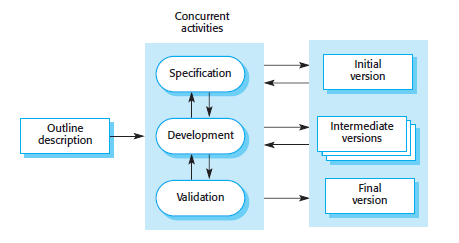
\includegraphics[width=0.70\linewidth]{img/incremental_development.png}
	\caption{Modello di sviluppo incrementale}
\end{figure}
\pagebreak

\section{Pianificazione}
Sulla base delle cadenza fissate in §1.6, la ripartizione delle attività di progetto avviene tramite:
\begin{itemize}
\item \textbf{Analisi};
\item \textbf{Consolidameto requisiti};
\item \textbf{Progettazione architetturale};
\item \textbf{Progettazione di dettaglio e codifica};
\item \textbf{Validazione e collaudo}.
\end{itemize}  

\subsection{Analisi}
\textit{Periodo: da 2020-03-16 a 2020-04-13} \\
La fase di analisi è suddivisa nel seguente modo:
\begin{itemize}
\item \textbf{Identificazione degli strumenti}: attività rivolta a determinare gli strumenti da utilizzare per le comunicazioni, stesura dei documenti, versionamento, sviluppo e verifica del sistema;
\item \textbf{Norme di Progetto}: sono l'insieme delle regole da seguire per lo svolgimento dei processi e la realizzazione del prodotto. Il documento \textit{Norme di Progetto}, è redatto dall'\textit{Amministratore};
\item \textbf{Studio di Fattibilità}: attività svolta dagli \textit{Analisti} con lo scopo di analizzare i capitolati, in linea generale, per stabilire quale di essi sia una proposta realizzabile. Inoltre è un'attivita propedeutica all'\textit{Analisi dei Requisiti};
\item \textbf{Analisi dei Requisiti}: sulla base dell'attività precedente, vengono identificati e definiti i requisiti del sistema. Come per il documento \textit{Studio di Fattibità}, anche \textit{Analisi dei Requisiti}, viene redatto dagli \textit{Analisti};
\item \textbf{Piano di Qualifica}: attività dell'\textit{Amministratore} e del \textit{Progettista} che si occupa di stabilire le metologie per garantire la qualità del prodotto. In particolar modo la seconda figura si focalizza sulla parte programmatica;
\item \textbf{Piano di Progetto}: il lavoro da svolgere viene suddiviso in compiti, risorse e attività da parte del \textit{Responsabile}, che ha anche il compito di calcolare il preventivo di periodo del progetto. Il tutto viene riportato sempre da parte del \textit{Responsabile} nel documento \textit{Piano di Progetto};
\item \textbf{Glossario}: tutti i vocaboli di difficile interpretazione vengono individuati riportati nel documento \textit{Glossario}.
\end{itemize}

\begin{figure}[H]
\centering
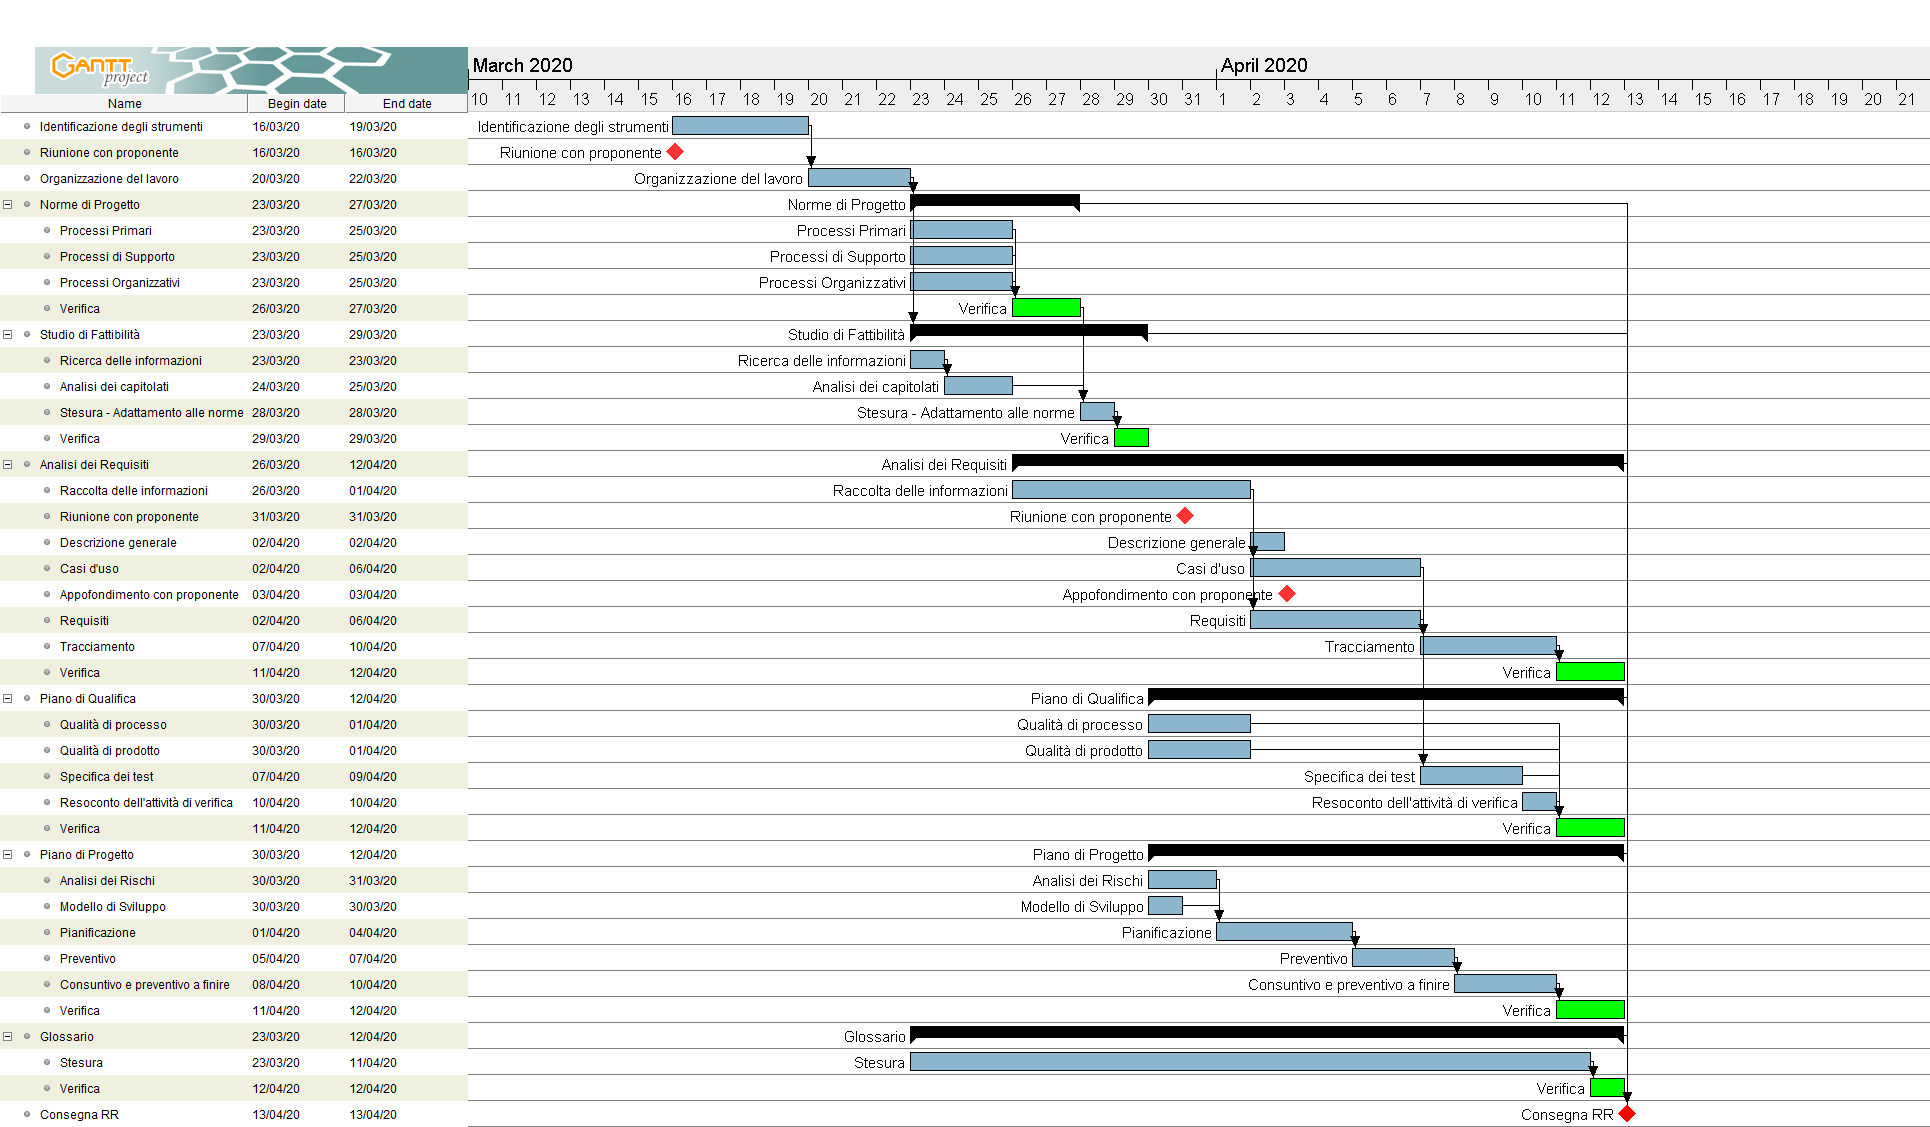
\includegraphics[scale=0.24]{./img/gantt/analisi.png}
\caption{Diagramma di Gantt della fase di Analisi}
\end{figure}

\subsection{Consolidamento dei requisiti}
\textit{Periodo: da 2020-04-14 a 2020-04-20}\\
La fase di consolidamento è così suddivisa:
\begin{itemize}
\item \textbf{Approfondimento personale}: attività intenta a fissare ed approfondire le informazioni riguardanti i requisiti evidenziati nella precedente fase;
\item \textbf{Raccolta informazioni}: raccolta delle informazioni necessarie per la presentazione;
\item \textbf{Stesura presentazione}: preparazione del materiale necessario alla presentazione del 2020-04-20;
\item \textbf{Studio personale}: tempo dedicato ai membri del gruppo, per studiare le informazioni contenute nella presentazione.
\end{itemize}

\begin{figure}[H]
\centering
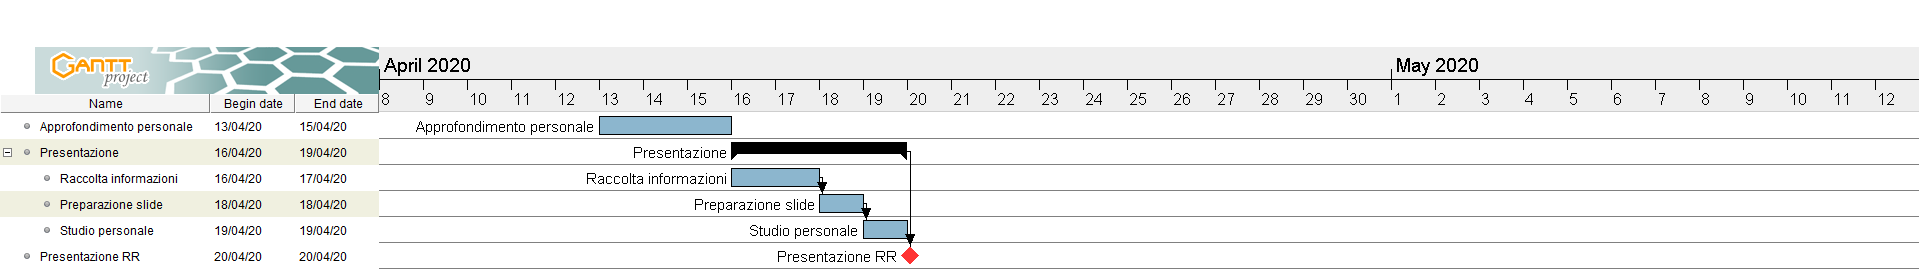
\includegraphics[scale=0.24]{./img/gantt/consolidamento_requisiti.png}
\caption{Diagramma di Gantt della fase di Consolidamento dei requisiti}
\end{figure}

\subsection{Progettazione architetturale}
\textit{Periodo: da 2020-04-21 a 2020-05-11}\\
Questa fase coincide con il giorno successivo alla presentazione del 2020-04-20 e termina con la consegna del materiale per la \textbf{Revisone di Progettazione}. La fase è così suddivisa in:
\begin{itemize}
\item \textbf{Technology Baseline}: vengono identificati i design pattern\glo necessari alloo sviluppo del sistema e verranno riportati nell'allegato tecnico insieme al tracciamento de requisiti. Inoltre viene presentato, al committente e al proponente, un prototipo per mezzo di un repository\glo;
\item \textbf{Incrementi e verifica}: sulla base dei feedback del committente e del proponente, viene migliorato e verificato il materiale del precedente rilascio.
\end{itemize}

\begin{figure}[H]
\centering
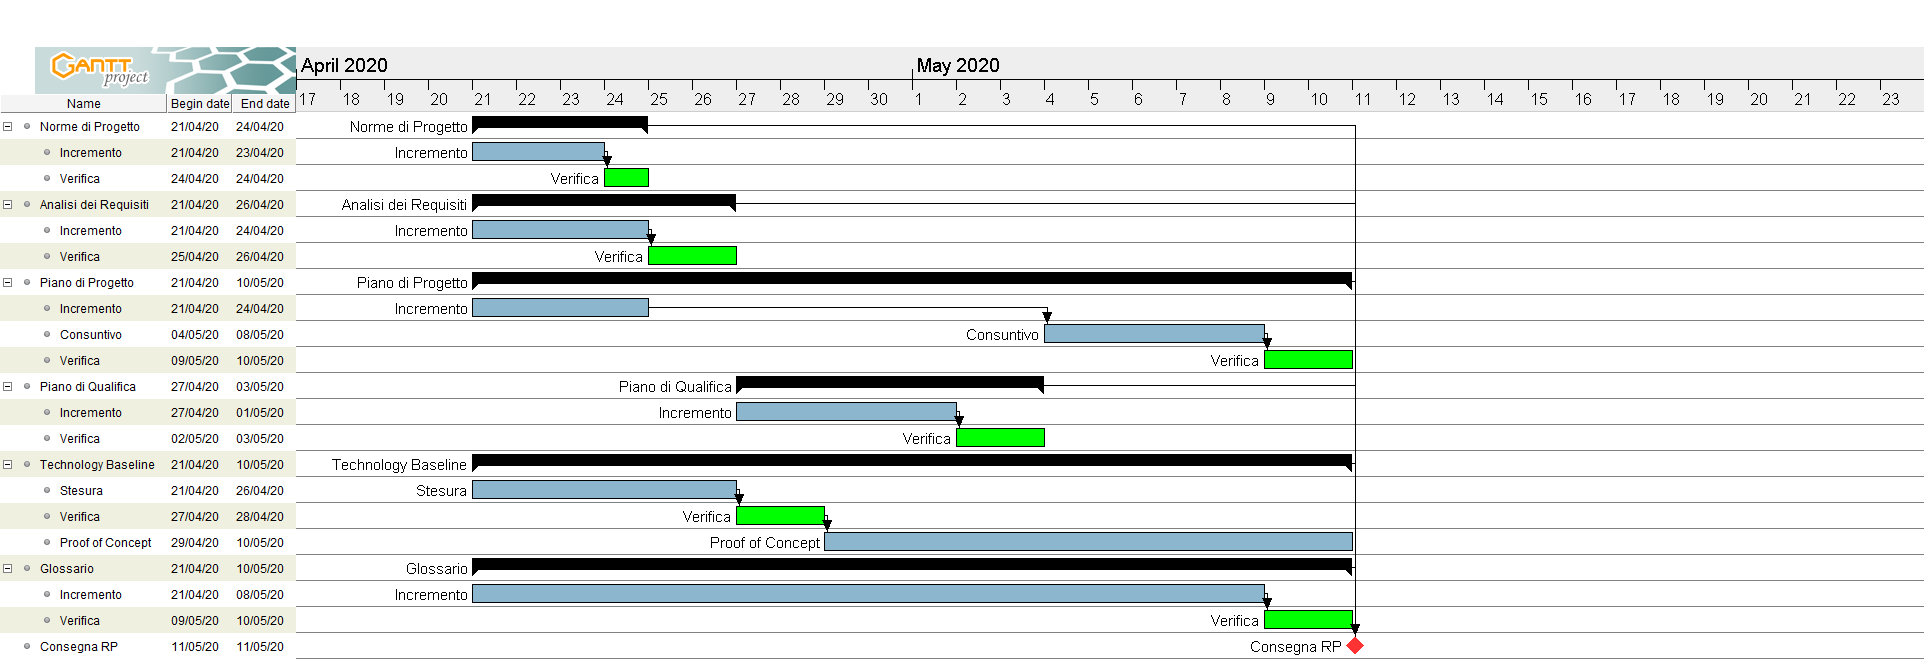
\includegraphics[scale=0.24]{./img/gantt/progettazione_architetturale.png}
\caption{Diagramma di Gantt della fase di Progettazione architetturale}
\end{figure}

\subsection{Progettazine di dettaglio e codifica}
\textit{Periodo: da 2020-05-11 a 2020-06-11}\\
Questa fase è compresa tra il giorno successivo alla presentazione del 2020-05-11 e la consegna della \textit{Revisione di Qualifica}.
\begin{itemize}
\item \textbf{Product Baseline}: le singole unità di cui è composta l'architettura definita nella \textit{Technology Baseline}, vengono ulteriormente analizzate;
\item \textbf{Incrementi e verifica}: sulla base dei feedback del committente e del proponente, viene migliorato e verificato il materiale del precedente rilascio.
\end{itemize}

\begin{figure}[H]
\centering
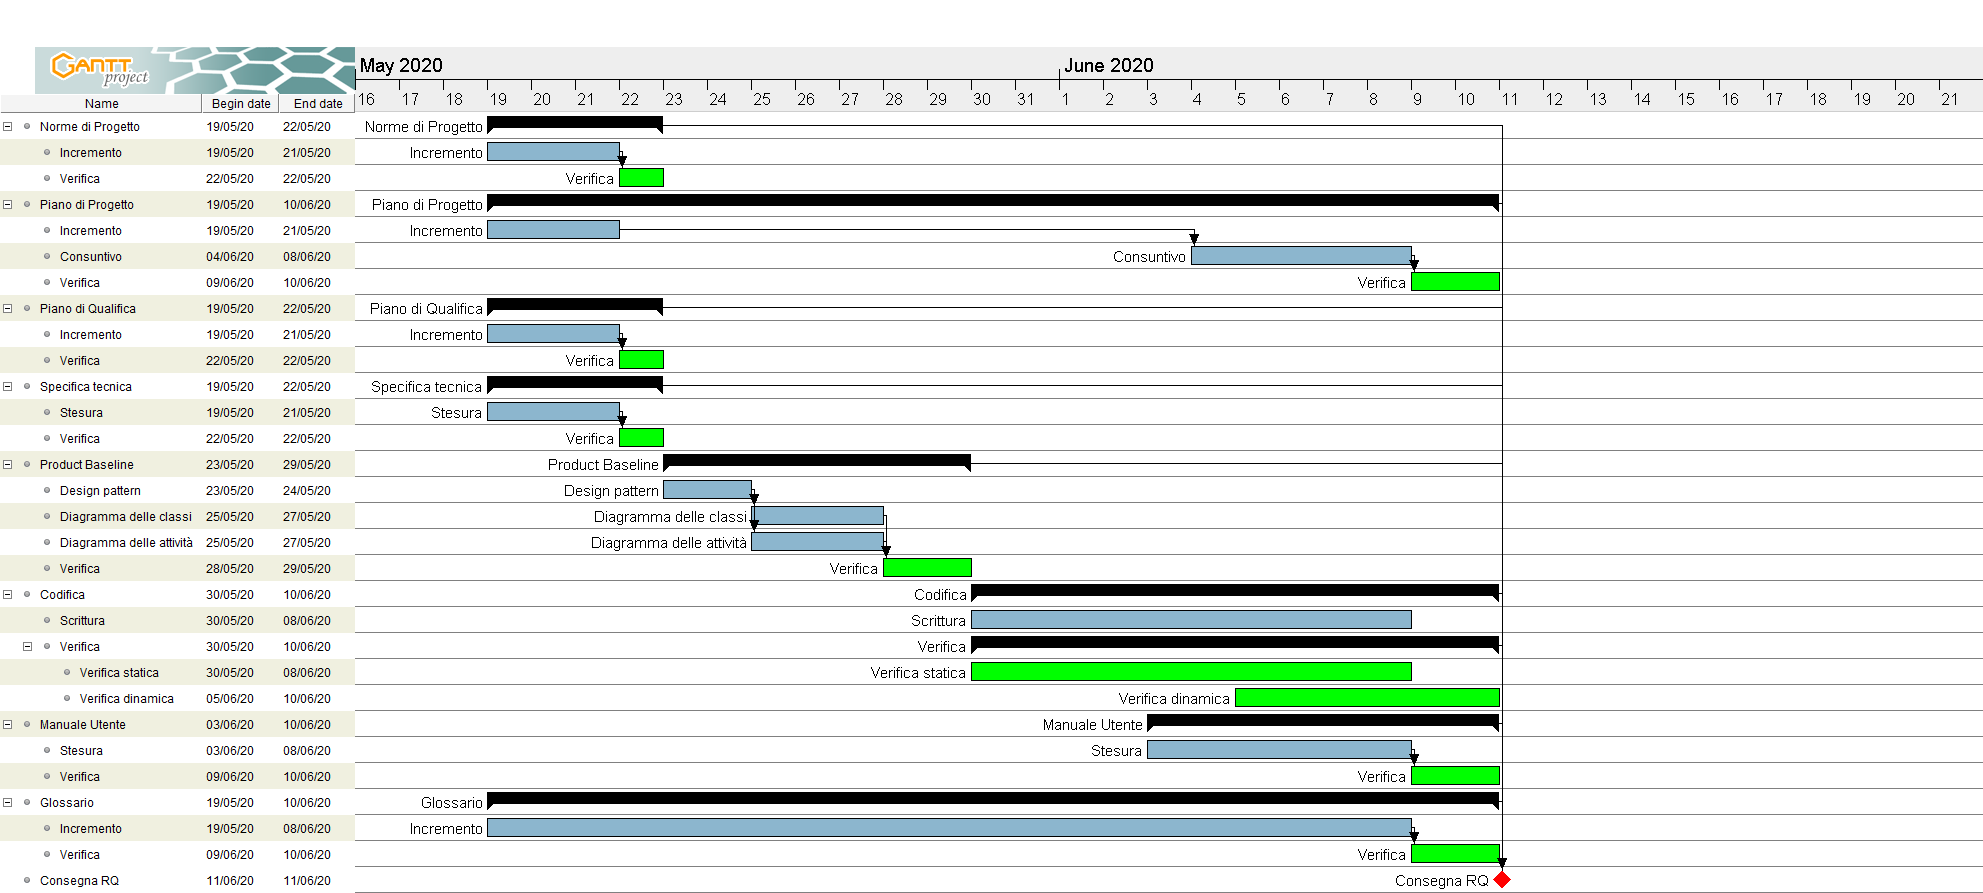
\includegraphics[scale=0.24]{./img/gantt/progettazione_dettaglio_codifica.png}
\caption{Diagramma di Gantt della fase di Progettazione di dettaglio e codifica}
\end{figure}

\subsection{Validazione e collaudo}
\textit{Periodo: da 2020-06-19 a 2020-07-06}\\
La seguente fase inizia il giorno seguente la \textit{Revisione di Qualifica} e termina con la consegna del materiale richiesto per la \textit{Revisione di Avanzamento}.
\begin{itemize}
\item \textbf{Incremento}: nel aso risltasse necessario vengono effetttuati miglioramenti sulla base di feedback;
\item \textbf{Validazione e collaudo}: la validazione effettua test sul prodotto, me tre la convalidazione controlla se viene rispettata la oerenza tra il prodotto e le specifiche evidenziate nel documento \textit{Analisi dei Requisiti};
\item \textbf{Manuale Sviluppatore}: viene redatto il documento \textit{Manuale dello Sviluppatore}, il quale contterrà le informazioni necessarie allo sviluppo, matenimento e manutenzione del prodotto;
\item \textbf{Manuale Utente}: viene redatto il documento \textit{Manuale dell'Utente}, il quale contterrà le informazioni necessarie all'utilizzo del prodotto.
\end{itemize}

\begin{figure}[H]
\centering
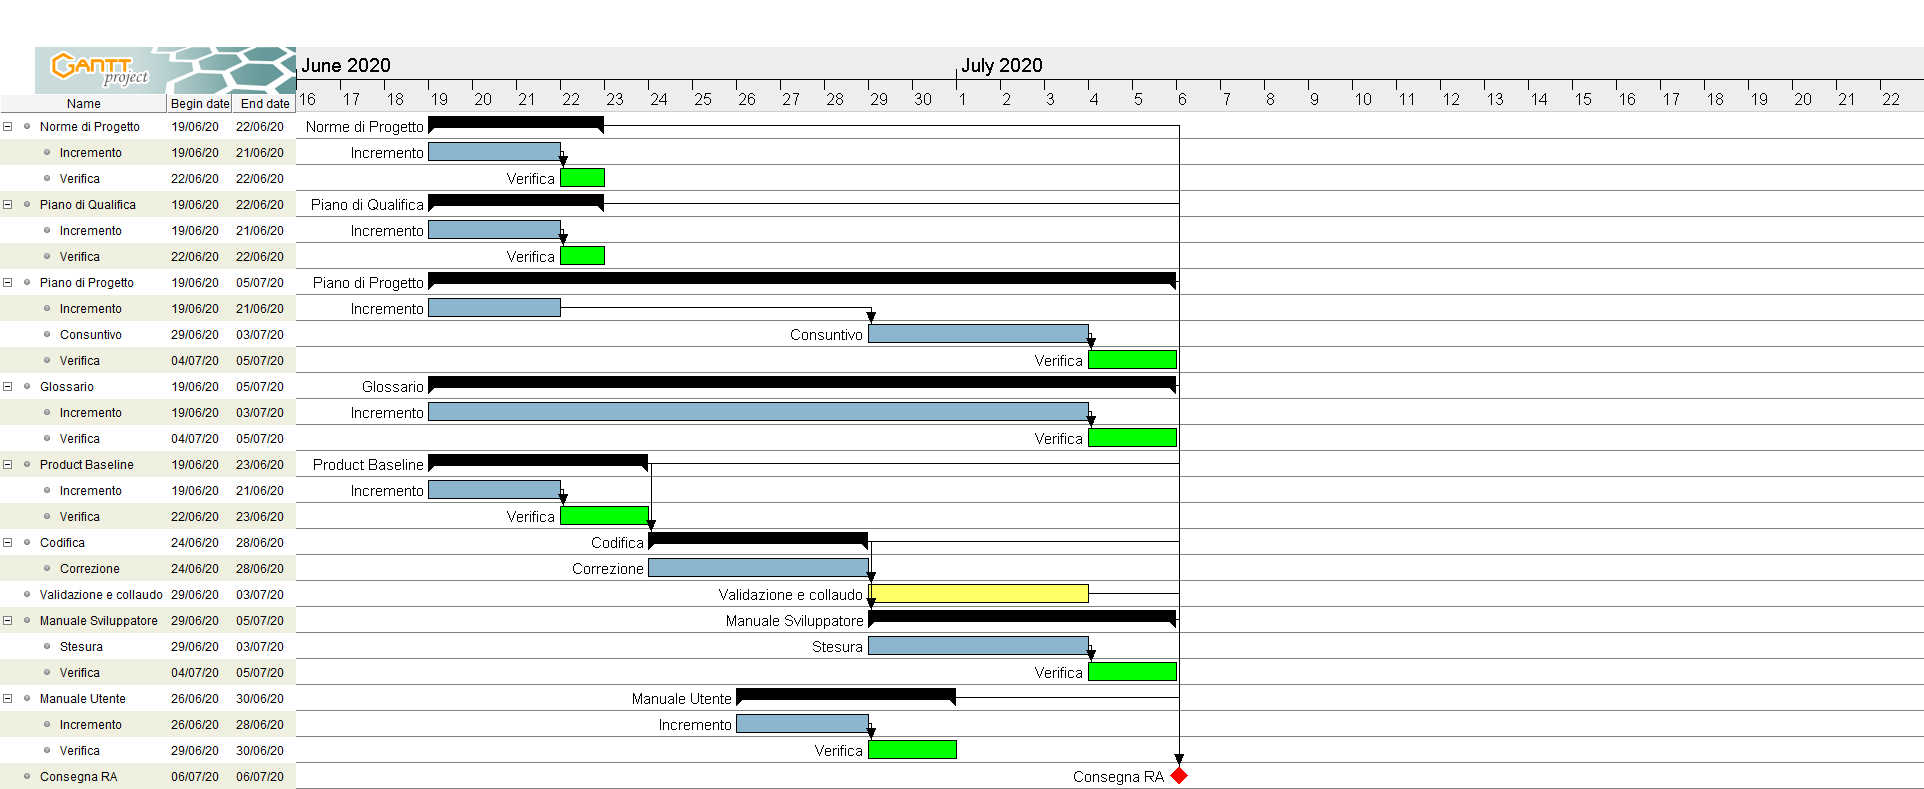
\includegraphics[scale=0.24]{./img/gantt/validazione_collaudo.png}
\caption{Diagramma di Gantt della fase di Validazione e collaudo}
\end{figure}
\pagebreak

\appendix %tutte le \section da questo documento in poi saranno numerate con lettere

\section{Preventivo di periodo}
Per facilitare la lettura delle tabelle, vengono utilizzate le seguenti sigle per identificare i diversi ruoli e per ognuno di essi vengono indicati i relativi costi/h: \begin{itemize}
\item \textbf{Re}: \textit{Responsabile} 30€/h;
\item \textbf{Am}: \textit{Amministratore} 20€/h;
\item \textbf{An}: \textit{Analista} 25€/h;
\item \textbf{Pt}: \textit{Progettista} 22€/h;
\item \textbf{Pm}: \textit{Programmatore} 15€/h;
\item \textbf{Ve}: \textit{Verificatore} 15€/h.
\end{itemize}
Inoltre, se le ore ricoperte in un determinato ruolo fossero nulle, la cella presenterà il simbolo "-" per indicarne l'assenza.
 
\subsection{Fase di Analisi}
\subsubsection{Distribuzione oraria}
In questa fase, i ruoli sono così suddivisi:
\begin{table}[H]
\centering\renewcommand{\arraystretch}{1.5}
\caption{Distribuzione delle ore nella fase di Analisi}
\vspace{0.2cm}
\begin{tabular}{ c | c | c | c | c | c | c | c }
\rowcolor{redafk}
\textcolor{white}{\textbf{Nominativo}} & \textcolor{white}{\textbf{Re}} &
\textcolor{white}{\textbf{Am}} & \textcolor{white}{\textbf{An}} &
\textcolor{white}{\textbf{Pt}} & \textcolor{white}{\textbf{Pm}} &
\textcolor{white}{\textbf{Ve}} & \textcolor{white}{\textbf{Totale}} \\
Simone Federico Bergamin & 6 & 7 & 20 & - & - & 9 & 42 \\
Alessandro Canesso & 8 & 6 & 16 & - & - & 12 & 42 \\
Victor Dutca & 9 & - & 15 & - & - & 16 & 40 \\
Fouad Farid & 7 & 7 & 12 & 6 & - & 8 & 40 \\
Simone Meneghin & - & 8 & 14 & 10 & - & 10 & 42 \\
Olivier Utshudi & - & 8 & 13 & 8 & - & 13 & 42 \\
Davide Zilio & 4 & 5 & 17 & - & - & 14 & 40 \\
\rowcolor{lastrowcolor}
\textbf{Ore totali ruolo} & \textbf{34} & \textbf{41} & \textbf{107} & \textbf{24} & \textbf{0} & \textbf{82} & \textbf{288} \\
\end{tabular}
\end{table}
 
\pagebreak
 
I dati ottenuti sono riassunti nel seguente istogramma:
\begin{figure}[H]
\centering
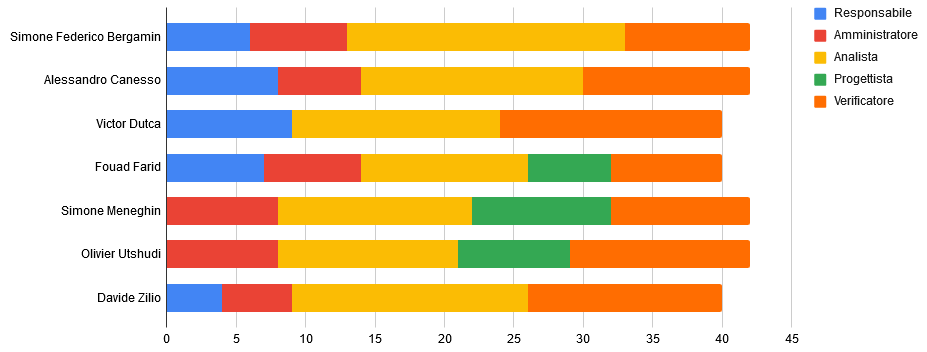
\includegraphics[scale=0.60]{img/grafici/tabella_fase_analisi.png}
\caption{Istogramma della ripartizione delle ore per ruolo nella fase di Analisi}
\end{figure}
 
\subsubsection{Prospetto economico}
In questa fase il costo per ogni ruolo è il seguente:
 
%tabella costi
\begin{table}[H]
\centering\renewcommand{\arraystretch}{1.5}
\caption{Prospetto dei costi nella fase di Analisi}
\vspace{0.2cm}
\begin{tabular}{ c | c | c  }
\rowcolor{redafk}
\textcolor{white}{\textbf{Ruolo}} & \textcolor{white}{\textbf{Ore}} &
\textcolor{white}{\textbf{Costo}}  \\
Responsabile & 34 & 1020€ \\
Amministratore & 41 & 820€ \\
Analista & 107 & 2675€ \\
Progettista & 24 & 528€ \\
Programmatore & 0 & 0€  \\
Verificatore & 82 & 1230€  \\
\rowcolor{lastrowcolor}
\textbf{Totale} & \textbf{288} & \textbf{6273€}  \\
\end{tabular}
\end{table}
 
I dati ottenuti sono riassunti nel seguente areogramma:
\begin{figure}[H]
\centering
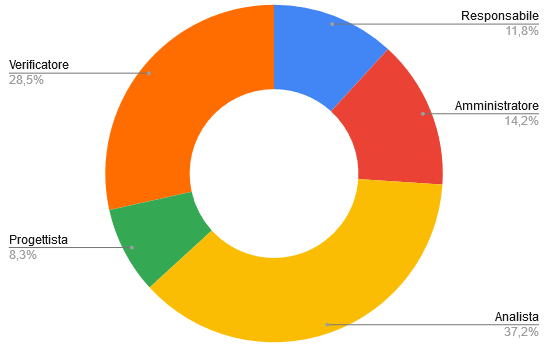
\includegraphics[scale=0.60]{img/grafici/torta_fase_analisi_prospetto_economico.png}
\caption{Areogramma della ripartizione dei costi per ruolo nella fase di Analisi}
\end{figure}
 
%--------------------------------------------------
 
\subsection{Fase di Progettazione architetturale}
\subsubsection{Distribuzione oraria}
In questa fase, i ruoli sono così suddivisi:
\begin{table}[H]
\centering\renewcommand{\arraystretch}{1.5}
\caption{Distribuzione delle ore nella fase di Progettazione architetturale}
\vspace{0.2cm}
\begin{tabular}{ c | c | c | c | c | c | c | c }
\rowcolor{redafk}
\textcolor{white}{\textbf{Nominativo}} & \textcolor{white}{\textbf{Re}} &
\textcolor{white}{\textbf{Am}} & \textcolor{white}{\textbf{An}} &
\textcolor{white}{\textbf{Pt}} & \textcolor{white}{\textbf{Pm}} &
\textcolor{white}{\textbf{Ve}} & \textcolor{white}{\textbf{Totale}} \\
Simone Federico Bergamin & - & - & 10 & 7 & 5 & 8 & 30 \\
Alessandro Canesso & - & 5 & - & 10 & 9 & 8 & 32 \\
Victor Dutca & 3 & 6 & 4 & 10 & 7 & - & 30 \\
Fouad Farid & - & 5 & - & 14 & - & 11 & 30 \\
Simone Meneghin & 6 & - & 9 & 10 & 7 & - & 32 \\
Olivier Utshudi & - & 4 & - & 10 & 6 & 12 & 32 \\
Davide Zilio & 3 & - & 13 & - & - & 14 & 30 \\
\rowcolor{lastrowcolor}
\textbf{Ore totali ruolo} & \textbf{12} & \textbf{20} & \textbf{36} & \textbf{61} & \textbf{34} & \textbf{53} & \textbf{216} \\
\end{tabular}
\end{table}
 
I dati ottenuti sono riassunti nel seguente istogramma:
\begin{figure}[H]
\centering
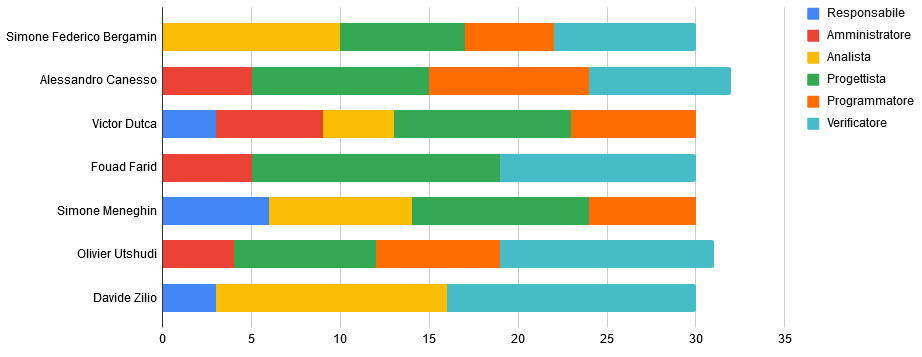
\includegraphics[scale=0.60]{img/grafici/tabella_fase_prog_architetturale.png}
\caption{Istogramma della ripartizione delle ore per ruolo nella fase di Progettazione architetturale}
\end{figure}
 
\subsubsection{Prospetto economico}
In questa fase il costo per ogni ruolo è il seguente:
 
%tabella costi
\begin{table}[H]
\centering\renewcommand{\arraystretch}{1.5}
\caption{Prospetto dei costi nella fase di Progettazione architetturale}
\vspace{0.2cm}
\begin{tabular}{ c | c | c  }
\rowcolor{redafk}
\textcolor{white}{\textbf{Ruolo}} & \textcolor{white}{\textbf{Ore}} &
\textcolor{white}{\textbf{Costo}}  \\
Responsabile & 12 & 360€ \\
Amministratore & 20 & 400€ \\
Analista & 36 & 900€ \\
Progettista & 61 & 1342€ \\
Programmatore & 34 & 510€  \\
Verificatore & 53 & 795€  \\
\rowcolor{lastrowcolor}
\textbf{Totale} & \textbf{216} & \textbf{4307€}  \\
\end{tabular}
\end{table}
 
I dati ottenuti sono riassunti nel seguente areogramma:
\begin{figure}[H]
\centering
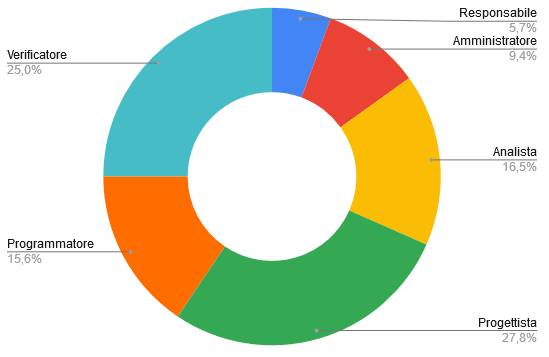
\includegraphics[scale=0.60]{img/grafici/torta_fase_prog_architetturale.png}
\caption{Areogramma della ripartizione dei costi per ruolo nella fase di Progettazione architetturale}
\end{figure}
 
%--------------------------------------------------
 
\subsection{Fase di Progettazione di dettaglio e codifica}
\subsubsection{Distribuzione oraria}
In questa fase, i ruoli sono così suddivisi:
\begin{table}[H]
\centering\renewcommand{\arraystretch}{1.5}
\caption{Distribuzione delle ore nella fase di Progettazione di dettaglio e codifica}
\vspace{0.2cm}
\begin{tabular}{ c | c | c | c | c | c | c | c }
\rowcolor{redafk}
\textcolor{white}{\textbf{Nominativo}} & \textcolor{white}{\textbf{Re}} &
\textcolor{white}{\textbf{Am}} & \textcolor{white}{\textbf{An}} &
\textcolor{white}{\textbf{Pt}} & \textcolor{white}{\textbf{Pm}} &
\textcolor{white}{\textbf{Ve}} & \textcolor{white}{\textbf{Totale}} \\
Simone Federico Bergamin & - & 6 & - & 12 & 18 & 12 & 48 \\
Alessandro Canesso & 4 & 3 & - & 10 & 18 & 11 & 46 \\
Victor Dutca & - & 8 & - & 10 & 20 & 10 & 48 \\
Fouad Farid & 4 & - & - & 12 & 20 & 12 & 48 \\
Simone Meneghin & 2 & - & - & 12 & 22 & 14 & 50 \\
Olivier Utshudi & 8 & - & - & 8 & 21 & 12 & 49 \\
Davide Zilio & - & 6 & - & 10 & 20 & 12 & 48 \\
\rowcolor{lastrowcolor}
\textbf{Ore totali ruolo} & \textbf{18} & \textbf{23} & \textbf{0} & \textbf{74} & \textbf{139} & \textbf{83} & \textbf{337} \\
\end{tabular}
\end{table}
 
I dati ottenuti sono riassunti nel seguente istogramma:
\begin{figure}[H]
\centering
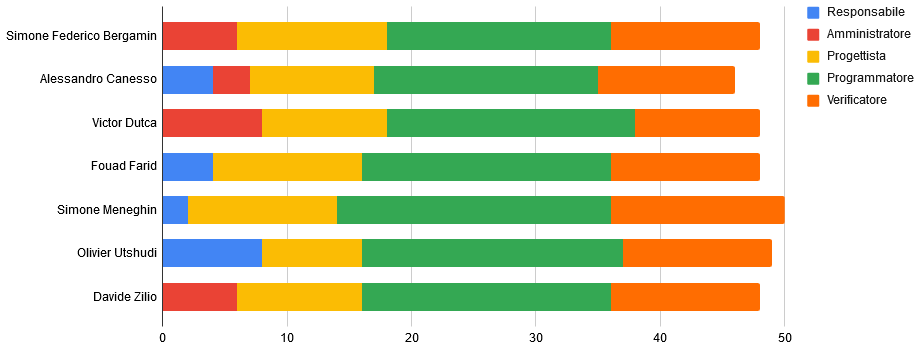
\includegraphics[scale=0.60]{img/grafici/tabella_fase_prog_cod.png}
\caption{Istogramma della ripartizione delle ore per ruolo nella fase di Progettazione di dettaglio e codifica}
\end{figure}
 
\subsubsection{Prospetto economico}
In questa fase il costo per ogni ruolo è il seguente:
 
%tabella costi
\begin{table}[H]
\centering\renewcommand{\arraystretch}{1.5}
\caption{Prospetto dei costi nella fase di Progettazione di dettaglio e codifica}
\vspace{0.2cm}
\begin{tabular}{ c | c | c  }
\rowcolor{redafk}
\textcolor{white}{\textbf{Ruolo}} & \textcolor{white}{\textbf{Ore}} &
\textcolor{white}{\textbf{Costo}}  \\
Responsabile & 18 & 540€ \\
Amministratore & 23 & 460€ \\
Analista & 0 & 0€ \\
Progettista & 74 & 1628€ \\
Programmatore & 139 & 2085€  \\
Verificatore & 83 & 1245€  \\
\rowcolor{lastrowcolor}
\textbf{Totale} & \textbf{337} & \textbf{5958€}  \\
\end{tabular}
\end{table}
 
I dati ottenuti sono riassunti nel seguente areogramma:
\begin{figure}[H]
\centering
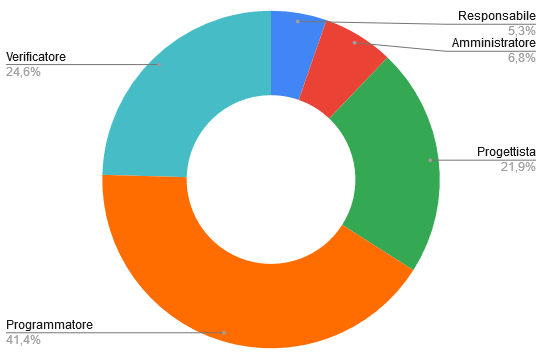
\includegraphics[scale=0.60]{img/grafici/torta_fase_prog_cod.png}
\caption{Areogramma della ripartizione dei costi per ruolo nella fase di Progettazione di dettaglio e codifica}
\end{figure}

%------------------------------------

\subsection{Fase di Validazione e collaudo}
\subsubsection{Distribuzione oraria}
In questa fase i ruoli sono così suddivisi:

%tabella ore
\begin{table}[H]
\centering\renewcommand{\arraystretch}{1.5}
\caption{Validazione e Collaudo}
\vspace{0.2cm}
\begin{tabular}{ c | c | c | c | c | c | c | c }
\rowcolor{redafk}
\textcolor{white}{\textbf{Nominativo}} & \textcolor{white}{\textbf{Re}} & 
\textcolor{white}{\textbf{Am}} & \textcolor{white}{\textbf{An}} &
\textcolor{white}{\textbf{Pt}} & \textcolor{white}{\textbf{Pm}} &
\textcolor{white}{\textbf{Ve}} & \textcolor{white}{\textbf{Totale}} \\
Simone Federico Bergamin 	& 5 	& - 	& - 	& - 	& 8 	& 12 	& 25 \\
Alessandro Canesso 			& 4 	& 4 	& - 	& - 	& - 	& 15 	& 23 \\
Victor Dutca 				& 5 	& - 	& - 	& - 	& 5 	& 15 	& 25 \\
Fouad Farid					& - 	& 6 	& - 	& - 	& 7 	& 12 	& 25 \\
Simone Meneghin 			& - 	& 9 	& - 	& - 	& - 	& 16 	& 25 \\
Olivier Utshudi 			& - 	& 4 	& - 	& 4 	& 5 	& 12 	& 25 \\
Davide Zilio 				& 6 	& - 	& - 	& 8 	& - 	& 11 	& 25 \\
\rowcolor{lastrowcolor}
\textbf{Ore totali ruolo} & \textbf{20} & \textbf{23} & \textbf{0} & \textbf{12} & \textbf{25} & \textbf{93} & \textbf{173} \\
\end{tabular}
\end{table}

I dati ottenuti sono riassunti nel seguente istogramma: 
\begin{figure}[H]
\centering
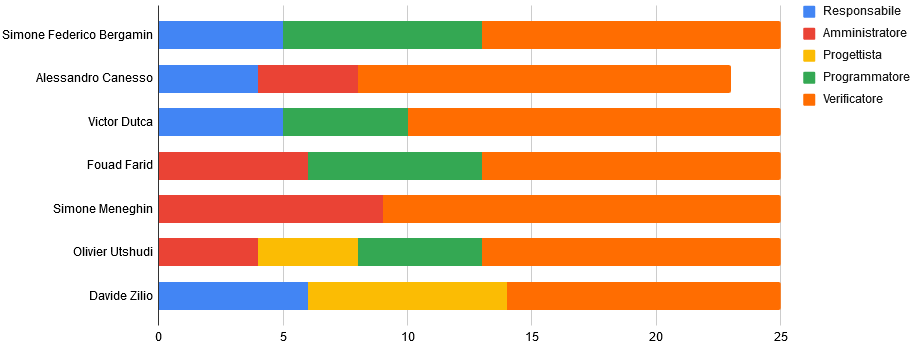
\includegraphics[scale=0.60]{img/grafici/tabella_fase_val_col.png}
\caption{Istogramma della ripartizione delle ore per ruolo nella fase di Validazione e collaudo}
\end{figure}

\subsubsection{Prospetto economico}
In questa fase il costo per ogni ruolo è il seguente:

%tabella costi
\begin{table}[H]
\centering\renewcommand{\arraystretch}{1.5}
\caption{Prospetto dei costi nella fase di Validazione e collaudo}
\vspace{0.2cm}
\begin{tabular}{ c | c | c  }
\rowcolor{redafk}
\textcolor{white}{\textbf{Ruolo}} & \textcolor{white}{\textbf{Ore}} & 
\textcolor{white}{\textbf{Costo}}  \\
Responsabile & 20 & 600€ \\
Amministratore & 23 & 460€ \\
Analista & - & - \\
Progettista	& 12 & 264€ \\
Programmatore & 25 & 375€  \\
Verificatore & 93 & 1395€  \\
\rowcolor{lastrowcolor}
\textbf{Totale} & \textbf{173} & \textbf{3094€}  \\
\end{tabular}
\end{table}

I dati ottenuti si possono riassumere nel seguente areogramma:
\begin{figure}[H]
\centering
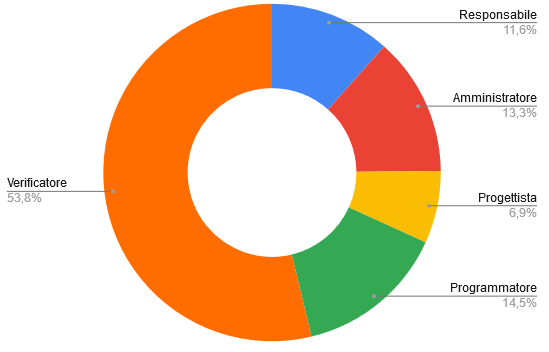
\includegraphics[scale=0.60]{img/grafici/torta_fase_val_col.png}
\caption{Areogramma della ripartizione dei costi per ruolo nella fase di Validazione e collaudo}
\end{figure}


\subsection{Riepilogo}
\subsubsection{Ore rendicontate con investimento}
\paragraph{Distribuzione oraria} \mbox{} \\ \mbox{} \\
Vengono riportate il totale delle ore del progetto in cui sono presenti le ore di investimento e le
ore rendicontate a carico del committente:

%tabella ore
\begin{table}[H]
\centering\renewcommand{\arraystretch}{1.5}
\caption{Distribuzione totale delle ore dell'intero progetto con investimento}
\vspace{0.2cm}
\begin{tabular}{ c | c | c | c | c | c | c | c }
\rowcolor{redafk}
\textcolor{white}{\textbf{Nominativo}} & \textcolor{white}{\textbf{Re}} & 
\textcolor{white}{\textbf{Am}} & \textcolor{white}{\textbf{An}} &
\textcolor{white}{\textbf{Pt}} & \textcolor{white}{\textbf{Pm}} &
\textcolor{white}{\textbf{Ve}} & \textcolor{white}{\textbf{Totale}} \\
Simone Federico Bergamin 	& 11 	& 13 	& 30 	& 19 	& 31 	& 41 	& 145 \\
Alessandro Canesso 			& 16 	& 18 	& 16 	& 20 	& 27 	& 46 	& 143 \\
Victor Dutca 				& 17	& 14 	& 19 	& 20 	& 32 	& 41 	& 143 \\
Fouad Farid					& 11	& 18 	& 12 	& 32 	& 27 	& 43 	& 143 \\
Simone Meneghin 			& 8 	& 17 	& 23 	& 32 	& 29 	& 40 	& 149 \\
Olivier Utshudi 			& 8 	& 16 	& 13 	& 30 	& 32 	& 49 	& 148 \\
Davide Zilio 				& 13 	& 11 	& 30 	& 18 	& 20 	& 51 	& 143 \\
\rowcolor{lastrowcolor}
\textbf{Ore totali ruolo} & \textbf{84} & \textbf{107} & \textbf{143} & \textbf{171} & \textbf{198} & \textbf{311} & \textbf{1014} \\
\end{tabular}
\end{table}

Una rappresentazione visiva della suddivisione oraria viene data dal seguente grafico:
\begin{figure}[H]
\centering
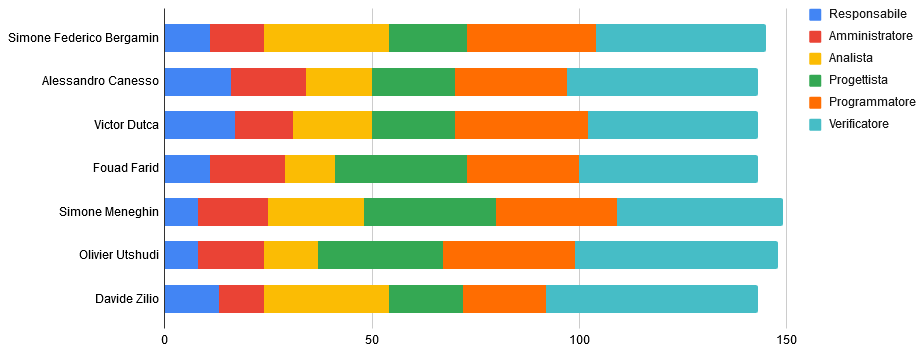
\includegraphics[scale=0.60]{img/grafici/tabella_tot_con_analisi.png}
\caption{Istogramma della ripartizione delle ore totali per ruolo con investimento}
\end{figure}

\paragraph{Prospetto economico} \mbox{} \\ \mbox{} \\
Il costo totale con investimento è riportato nella seguente tabella:

%tabella costi
\begin{table}[H]
\centering\renewcommand{\arraystretch}{1.5}
\caption{Costi totali con investimento}
\vspace{0.2cm}
\begin{tabular}{ c | c | c  }
\rowcolor{redafk}
\textcolor{white}{\textbf{Ruolo}} & \textcolor{white}{\textbf{Ore}} & 
\textcolor{white}{\textbf{Costo}}  \\
Responsabile & 84 & 2520€ \\
Amministratore & 107 & 2140€ \\
Analista & 143 & 3575€ \\
Progettista	& 171 & 3762€ \\
Programmatore & 198 & 2970€  \\
Verificatore & 311 & 4665€  \\
\rowcolor{lastrowcolor}
\textbf{Totale} & \textbf{1014} & \textbf{19632€}  \\
\end{tabular}
\end{table}

I dati ottenuti si possono riassumere nel seguente areogramma:
\begin{figure}[H]
\centering
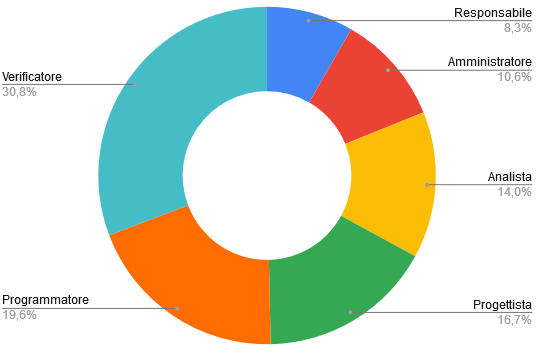
\includegraphics[scale=0.60]{img/grafici/torta_tot_con_analisi.png}
\caption{Areogramma della ripartizione dei costi totali per ruolo con investimento}
\end{figure}

\subsubsection{Ore rendicontate senza investimento}
\paragraph{Distribuzione oraria} \mbox{} \\ \mbox{} \\
Le ore rendicontate sono riassunte nella seguente tabella:

%tabella ore
\begin{table}[H]
\centering\renewcommand{\arraystretch}{1.5}
\caption{Distribuzione totale delle ore dell'intero progetto senza investimento}
\vspace{0.2cm}
\begin{tabular}{ c | c | c | c | c | c | c | c }
\rowcolor{redafk}
\textcolor{white}{\textbf{Nominativo}} & \textcolor{white}{\textbf{Re}} & 
\textcolor{white}{\textbf{Am}} & \textcolor{white}{\textbf{An}} &
\textcolor{white}{\textbf{Pt}} & \textcolor{white}{\textbf{Pm}} &
\textcolor{white}{\textbf{Ve}} & \textcolor{white}{\textbf{Totale}} \\
Simone Federico Bergamin 	& 5 	& 6 	& 10	& 19	& 31	& 32 	& 103 \\
Alessandro Canesso 			& 8 	& 12	& - 	& 20	& 27	& 34 	& 101 \\
Victor Dutca 				& 8 	& 14	& 4 	& 20	& 32	& 25 	& 103 \\
Fouad Farid					& 4 	& 11	& - 	& 26	& 27	& 35 	& 103 \\
Simone Meneghin 			& 8 	& 9 	& 9 	& 22	& 29	& 30 	& 107 \\
Olivier Utshudi 			& 8 	& 8 	& - 	& 22	& 32	& 36 	& 106 \\
Davide Zilio 				& 9 	& 6 	& 13	& 18	& 20	& 37 	& 103 \\
\rowcolor{lastrowcolor}
\textbf{Ore totali ruolo} & \textbf{50} & \textbf{66} & \textbf{36} & \textbf{147} & \textbf{198} & \textbf{229} & \textbf{726} \\
\end{tabular}
\end{table}

Una rappresentazione visiva della suddivisione oraria viene data dal seguente grafico:
\begin{figure}[H]
\centering
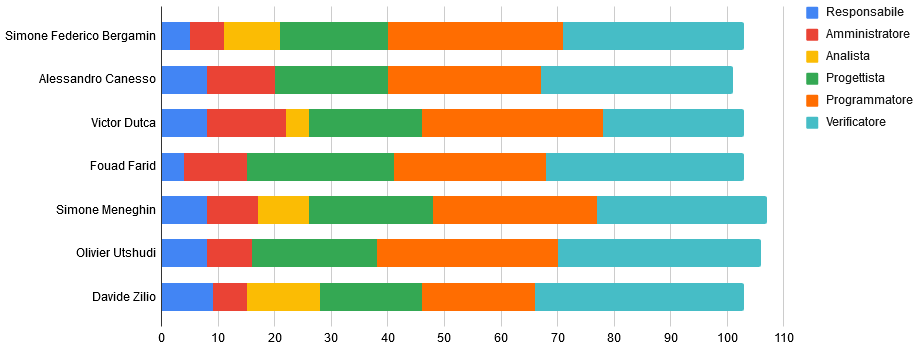
\includegraphics[scale=0.60]{img/grafici/tabella_tot_no_analisi.png}
\caption{Istogramma della ripartizione delle ore totali per ruolo con investimento}
\end{figure}

\paragraph{Prospetto economico} \mbox{} \\ \mbox{} \\
Il costo totale senza investimento è riportato nella seguente tabella:

%tabella costi
\begin{table}[H]
\centering\renewcommand{\arraystretch}{1.5}
\caption{Costi totali senza investimento}
\vspace{0.2cm}
\begin{tabular}{ c | c | c  }
\rowcolor{redafk}
\textcolor{white}{\textbf{Ruolo}} & \textcolor{white}{\textbf{Ore}} & 
\textcolor{white}{\textbf{Costo}}  \\
Responsabile & 50 & 1500€ \\
Amministratore & 66 & 1320€ \\
Analista & 36 & 900€ \\
Progettista	& 147 & 3234€ \\
Programmatore & 198 & 2970€  \\
Verificatore & 229 & 3435€  \\
\rowcolor{lastrowcolor}
\textbf{Totale} & \textbf{729} & \textbf{13359€}  \\
\end{tabular}
\end{table}

I dati ottenuti si possono riassumere nel seguente areogramma:
\begin{figure}[H]
\centering
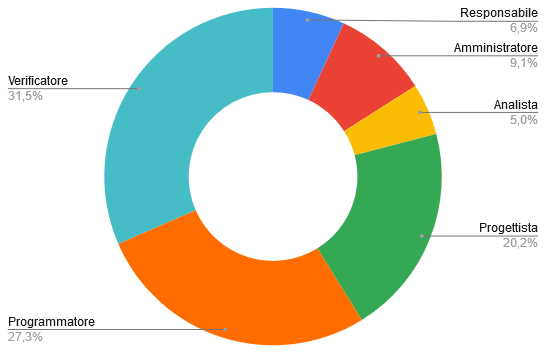
\includegraphics[scale=0.60]{img/grafici/torta_tot_no_analisi.png}
\caption{Areogramma della ripartizione dei costi totali per ruolo senza investimento}
\end{figure}

\subsection{Conclusioni}
Il costo totale preventivato per il progetto è 13.359,00€
\pagebreak

\section{Consuntivo di periodo}
Di seguito verranno indicate le spese effettivamente sostenute da ogni ruolo. Il bilancio di consuntivo potrà risultare: \begin{itemize}
\item \textbf{Positivo}: se il preventivo supera il consuntivo;
\item \textbf{Pari}: se preventivo e consuntivo sono uguali;
\item \textbf{Negativo}: se il consuntivo supera il preventivo.
\end{itemize}

\subsection{Analisi}
%tabella costi
\begin{table}[H]
\centering\renewcommand{\arraystretch}{1.5}
\caption{Consuntivo del periodo di Analisi}
\vspace{0.2cm}
\begin{tabular}{ c | c | c  }
\rowcolor{redafk}
\textcolor{white}{\textbf{Ruolo}} & \textcolor{white}{\textbf{Ore}} & 
\textcolor{white}{\textbf{Costo}}  \\
Responsabile & 34 & 1020€ \\
Amministratore & 41 (+13) & 820€ (+260€) \\
Analista & 107 (+8) & 2675€ (+200€) \\
Progettista	& 24 & 528€  \\
Programmatore & 0 & 0€  \\
Verificatore & 82 (+9) & 1230€ (+135€)  \\
\textbf{Totale preventivo} & \textbf{288} & \textbf{6273€}  \\
\textbf{Totale consuntivo} & \textbf{318} & \textbf{6868€}  \\
\rowcolor{lastrowcolor}
\textbf{Differenza} & \textbf{30} & \textbf{+595€}  \\
\end{tabular}
\end{table}

\subsubsection{Conclusioni}
Come emerge dai dati riportati nella tabella soprastante è stato necessario investire più tempo del previsto nei ruoli di \textit{Amministratore}, \textit{Analista} e \textit{Verificatore}. Per questo motivo il bilancio risultante è negativo. Le cause di tali ritardi sono riportate di seguito:
\begin{itemize}
\item \textbf{\textit{Amministratore}}: è servito più tempo del previsto per riuscire ad individuare i software più adatti per la gestione del progetto e per la loro  configurazione. Inoltre sono state aggiunte ed aggiornate alcune sezioni nelle \textit{Norme di Progetto}, necessarie al chiarimento di alcune problematiche sorte durante la stesura dei documenti;
\item \textbf{\textit{Analista}}: alcuni requisiti si sono rivelati di non facile comprensione, e sono state necessarie più ore di lavoro per la discussione interna tra gli \textit{analisti} ed esterna con il proponente;
\item \textbf{\textit{Verificatore}}: l’aggiunta di nuove sezioni nelle \textit{Norme di Progetto} e l'inesperienza dei membri hanno implicato un maggiore lavoro anche per questo ruolo.
\end{itemize}
\pagebreak

%comandi per inserimento tabelle (corrette e funzionanti)
\begin{comment}
%definizione colori per tabelle (tranne copertina)
\definecolor{redafk}{RGB}{255, 71, 87}
\definecolor{grey2}{RGB}{204, 204, 204}
\definecolor{lastrowcolor}{RGB}{156, 198, 214}
\definecolor{greyRowafk}{RGB}{234, 234, 234}
\rowcolors{2}{grey2}{greyRowafk}
\renewcommand{\arraystretch}{1.5}


%tabella ore
\begin{table}[H]
\centering\renewcommand{\arraystretch}{1.5}
\caption{Fase di Analisi}
\vspace{0.2cm}
\begin{tabular}{ c | c | c | c | c | c | c | c }
\rowcolor{redafk}
\textcolor{white}{\textbf{Nominativo}} & \textcolor{white}{\textbf{Re}} & 
\textcolor{white}{\textbf{Am}} & \textcolor{white}{\textbf{An}} &
\textcolor{white}{\textbf{Pt}} & \textcolor{white}{\textbf{Pr}} &
\textcolor{white}{\textbf{Ve}} & \textcolor{white}{\textbf{Totale}} \\
Simone Federico Bergamin & 6 & 6 & 18 & - & - & 9 & 39 \\
Alessandro Canesso & 6 & 5 & 18 & - & - & 10 & 39 \\
Victor Dutca & 10 & - & 15 & - & - & 14 & 39 \\
Fouad Farid	& 6 & 9 & 16 & - & - & 8 & 39 \\
Simone Meneghin & - & 7 & 10 & 12 & - & 10 & 39 \\
Olivier Utshudi & - & 8 & 10 & 8 & - & 13 & 39 \\
Davide Zilio & 4 & 5 & 16 & - & - & 14 & 39 \\
\rowcolor{lastrowcolor}
\textbf{Ore totali ruolo} & \textbf{32} & \textbf{40} & \textbf{103} & \textbf{20} & \textbf{0} & \textbf{78} & \textbf{273} \\
\end{tabular}
\end{table}


%tabella costi
\begin{table}[H]
\centering\renewcommand{\arraystretch}{1.5}
\caption{Fase di Analisi}
\vspace{0.2cm}
\begin{tabular}{ c | c | c  }
\rowcolor{redafk}
\textcolor{white}{\textbf{Ruolo}} & \textcolor{white}{\textbf{Ore}} & 
\textcolor{white}{\textbf{Costo}}  \\
Responsabile & 32 & 960€ \\
Amministratore & 40 & 800€ \\
Analista & 103 & 2575€ \\
Progettista	& 20 & 440€ \\
Programmatore & 0 & 0€  \\
Verificatore & 78 & 1170€  \\
\rowcolor{lastrowcolor}
\textbf{Totale} & \textbf{273} & \textbf{5945€}  \\
\end{tabular}
\end{table}

%definizione colori per tabelle (tranne copertina)
\definecolor{redafk}{RGB}{255, 71, 87}
\definecolor{grey2}{RGB}{204, 204, 204}
\definecolor{lastrowcolor}{RGB}{156, 198, 214}
\definecolor{greyRowafk}{RGB}{234, 234, 234}
\rowcolors{2}{grey2}{greyRowafk}
\renewcommand{\arraystretch}{1.5}


%tabella ore fase di Prog Architetturale
\begin{comment}
BASE PER TUTTI: 30 ORE
Canesso: +2 ore perchè sa che dopo dovrà farne di meno (tanti arretrati)
Utshudi & Meneghin: +2 ore perchè meno arretrati
\end{comment}

\begin{table}[H]
\centering\renewcommand{\arraystretch}{1.5}
\caption{Fase di Analisi}
\vspace{0.2cm}
\begin{tabular}{ c | c | c | c | c | c | c | c }
\rowcolor{redafk}
\textcolor{white}{\textbf{Nominativo}} & \textcolor{white}{\textbf{Re}} & 
\textcolor{white}{\textbf{Am}} & \textcolor{white}{\textbf{An}} &
\textcolor{white}{\textbf{Pt}} & \textcolor{white}{\textbf{Pr}} &
\textcolor{white}{\textbf{Ve}} & \textcolor{white}{\textbf{Totale}} \\
Simone Federico Bergamin & - & - & 10 & 7 & 5 & 8 & 30 \\
Alessandro Canesso & - & 5 & - & 10 & 9 & 8 & 32 \\
Victor Dutca & 3 & 6 & 4 & 10 & 7 & - & 30 \\
Fouad Farid	& - & 5 & - & 14 & - & 11 & 30 \\
Simone Meneghin & 6 & - & 9 & 10 & 7 & - & 32 \\
Olivier Utshudi & - & 4 & - & 10 & 6 & 12 & 32 \\
Davide Zilio & 3 & - & 13 & - & - & 14 & 30 \\
\rowcolor{lastrowcolor}
\textbf{Ore totali ruolo} & \textbf{12} & \textbf{20} & \textbf{36} & \textbf{61} & \textbf{34} & \textbf{53} & \textbf{216} \\
\end{tabular}
\end{table}


%tabella costi
\begin{table}[H]
\centering\renewcommand{\arraystretch}{1.5}
\caption{Fase di Analisi}
\vspace{0.2cm}
\begin{tabular}{ c | c | c  }
\rowcolor{redafk}
\textcolor{white}{\textbf{Ruolo}} & \textcolor{white}{\textbf{Ore}} & 
\textcolor{white}{\textbf{Costo}}  \\
Responsabile & 12 & 360€ \\
Amministratore & 20 & 400€ \\
Analista & 36 & 900€ \\
Progettista	& 61 & 1342€ \\
Programmatore & 34 & 510€  \\
Verificatore & 53 & 795€  \\
\rowcolor{lastrowcolor}
\textbf{Totale} & \textbf{216} & \textbf{4307€}  \\
\end{tabular}
\end{table}

%definizione colori per tabelle (tranne copertina)
\definecolor{redafk}{RGB}{255, 71, 87}
\definecolor{grey2}{RGB}{204, 204, 204}
\definecolor{lastrowcolor}{RGB}{156, 198, 214}
\definecolor{greyRowafk}{RGB}{234, 234, 234}
\rowcolors{2}{grey2}{greyRowafk}
\renewcommand{\arraystretch}{1.5}

%tabella ore fase di Prog Dettaglio e Codifica
\begin{comment}
BASE PER TUTTI: 48 ORE
Canesso: -2 ore perchè deve studiare per gli arretrati (4)
Utshudi: +1 ore perchè meno arretrati (-1 ora rispetto a Meneghin perchè il proj di TecWeb porta via tempo)
Meneghin: +2 ore (solo analisi)
\end{comment}

\begin{table}[H]
\centering\renewcommand{\arraystretch}{1.5}
\caption{Fase di Analisi}
\vspace{0.2cm}
\begin{tabular}{ c | c | c | c | c | c | c | c }
\rowcolor{redafk}
\textcolor{white}{\textbf{Nominativo}} & \textcolor{white}{\textbf{Re}} & 
\textcolor{white}{\textbf{Am}} & \textcolor{white}{\textbf{An}} &
\textcolor{white}{\textbf{Pt}} & \textcolor{white}{\textbf{Pr}} &
\textcolor{white}{\textbf{Ve}} & \textcolor{white}{\textbf{Totale}} \\
Simone Federico Bergamin & - & 6 & - & 12 & 18 & 12 & 48 \\
Alessandro Canesso & 4 & 3 & - & 10 & 18 & 11 & 46 \\
Victor Dutca & - & 8 & - & 10 & 20 & 10 & 48 \\
Fouad Farid	& 4 & - & - & 12 & 20 & 12 & 48 \\
Simone Meneghin & 2 & - & - & 12 & 22 & 14 & 50 \\
Olivier Utshudi & 8 & - & - & 8 & 21 & 12 & 49 \\
Davide Zilio & - & 6 & - & 10 & 20 & 12 & 48 \\
\rowcolor{lastrowcolor}
\textbf{Ore totali ruolo} & \textbf{18} & \textbf{23} & \textbf{0} & \textbf{74} & \textbf{139} & \textbf{83} & \textbf{337} \\
\end{tabular}
\end{table}


%tabella costi
\begin{table}[H]
\centering\renewcommand{\arraystretch}{1.5}
\caption{Fase di Analisi}
\vspace{0.2cm}
\begin{tabular}{ c | c | c  }
\rowcolor{redafk}
\textcolor{white}{\textbf{Ruolo}} & \textcolor{white}{\textbf{Ore}} & 
\textcolor{white}{\textbf{Costo}}  \\
Responsabile & 18 & 540€ \\
Amministratore & 23 & 460€ \\
Analista & 0 & 0€ \\
Progettista	& 74 & 1628€ \\
Programmatore & 139 & 2085€  \\
Verificatore & 83 & 1245€  \\
\rowcolor{lastrowcolor}
\textbf{Totale} & \textbf{337} & \textbf{5958€}  \\
\end{tabular}
\end{table}

\end{comment}

\section{Organigramma}
\subsection{Redazione} 
\begin{table}[H]
	\begin{center}
	\begin{tabular}{ c c C{6.6cm} }
		\rowcolor{redafk}
		\textcolor{white}{\textbf{Nominativo}} & \textcolor{white}{\textbf{Data di redazione}} & \textcolor{white}{\textbf{Firma}} \\
		Olivier Utshudi & 2020-04-10 & 
\includegraphics[scale=0.3, width=0.25\textwidth]{img/firme/outshudi.png}\\
		Simone Meneghin & 2020-04-10 & 
\includegraphics[scale=0.3, width=0.25\textwidth]{img/firme/meneghin.png}\\
		Davide Zilio & 2020-04-10 & 
\includegraphics[scale=0.2, width=0.2\textwidth]{img/firme/zilio.png}\\
	\end{tabular}
	\end{center}	
\end{table}

\subsection{Approvazione} 
\begin{table}[H]
	\begin{center}
	\begin{tabular}{ c c C{6cm} }
		\rowcolor{redafk}
		\textcolor{white}{\textbf{Nominativo}} & \textcolor{white}{\textbf{Data di approvazione}} & \textcolor{white}{\textbf{Firma}} \\
		Victor Dutca & 2020-04-12 &  
\includegraphics[scale=0.3, width=0.25\textwidth]{img/firme/dutca.png} \\
		Tullio Vardanega &  & \\
		Riccardo Cardin &  & \\
	\end{tabular}
	\end{center}	
\end{table}

\subsection{Accettazione dei componenti}
\begin{table}[H]	
	\begin{center}
	\begin{tabular}{ C{5cm} C{4cm} C{6cm}}
		\rowcolor{redafk}
		\textcolor{white}{\textbf{Nominativo}} & \textcolor{white}{\textbf{Data di accettazione}} & \textcolor{white}{\textbf{Firma}} \\
		Simone Federico Bergamin & 2020-03-09 & 
\includegraphics[scale=0.4]{img/firme/bergamin.png}\\
		Alessandro Canesso & 2020-03-09 & 
\includegraphics[scale=0.3, width=0.25\textwidth]{img/firme/canesso.png}\\
		Victor Dutca & 2020-03-09 & 
\includegraphics[scale=0.3, width=0.25\textwidth]{img/firme/dutca.png}\\
		Fouad Farid & 2020-03-09 & 
\includegraphics[scale=0.2, width=0.2\textwidth]{img/firme/farid.png}\\
		Simone Meneghin & 2020-03-09 & 
\includegraphics[scale=0.2, width=0.2\textwidth]{img/firme/meneghin.png}\\
		Olivier Utshudi & 2020-03-09 & 
\includegraphics[scale=0.3, width=0.25\textwidth]{img/firme/outshudi.png}\\
		Davide Zilio & 2020-03-09 & 
\includegraphics[scale=0.2, width=0.2\textwidth]{img/firme/zilio.png}\\
	\end{tabular}
	\end{center}
\end{table}

\subsection{Componenti}
\begin{table}[H]	
	\begin{center}
	\begin{tabular}{ C{4cm} C{3cm} C{8cm} }
		\rowcolor{redafk}
		\textcolor{white}{\textbf{Nominativo}} & \textcolor{white}{\textbf{Matricola}} & \textcolor{white}{\textbf{Indirizzo email}} \\
		Simone Federico Bergamin & 1144724  & simonefederico.bergamin@studenti.unipd.it \\
		Alessandro Canesso & 1122701 & alessandro.canesso@studenti.unipd.it\\
		Victor Dutca & 1122137 & victor.dutca@studenti.unipd.it\\
		Fouad Farid & 1122195 & fouad.farid@studenti.unipd.it\\
		Simone Meneghin & 1174926 & simone.meneghin@studenti.unipd.it\\
		Olivier Utshudi & 1143556 & olivier.utshudi@studenti.unipd.it\\
		Davide Zilio & 1149807 & davide.zilio.3@studenti.unipd.it\\
	\end{tabular}
	\end{center}
\end{table}
\pagebreak


\end{document}